\appendix
\chapter{Appendices}

\section{Appendix A: System Diagrams}

\subsection{Use Case Diagram}
\begin{figure}[H]
    \centering
    \includegraphics[width=\textwidth]{images/usecase.png}
    \caption{Use Case Diagram CoWriteIA}
    \label{fig:usecase}
\end{figure}

\subsection{Activity Diagram}
\begin{figure}[H]
    \centering
    \includegraphics[width=\textwidth]{images/activity 3.png}
    \caption{Activity Diagram}
    \label{fig:activity}
\end{figure}

\section{Appendix B: Architecture Diagram}

\subsection{CoWriteIA Detailed Architecture Diagram}
\begin{figure}[H]
    \centering
    \includegraphics[width=\textwidth]{images/architecture.png}
    \caption{CoWriteIA Multi-Tier Architecture Diagram}
    \label{fig:cowriteia-architecture}
\end{figure}

\section{Appendix C: User Interface Screenshots}

\subsection{Landing Page}
\begin{figure}[H]
    \centering
    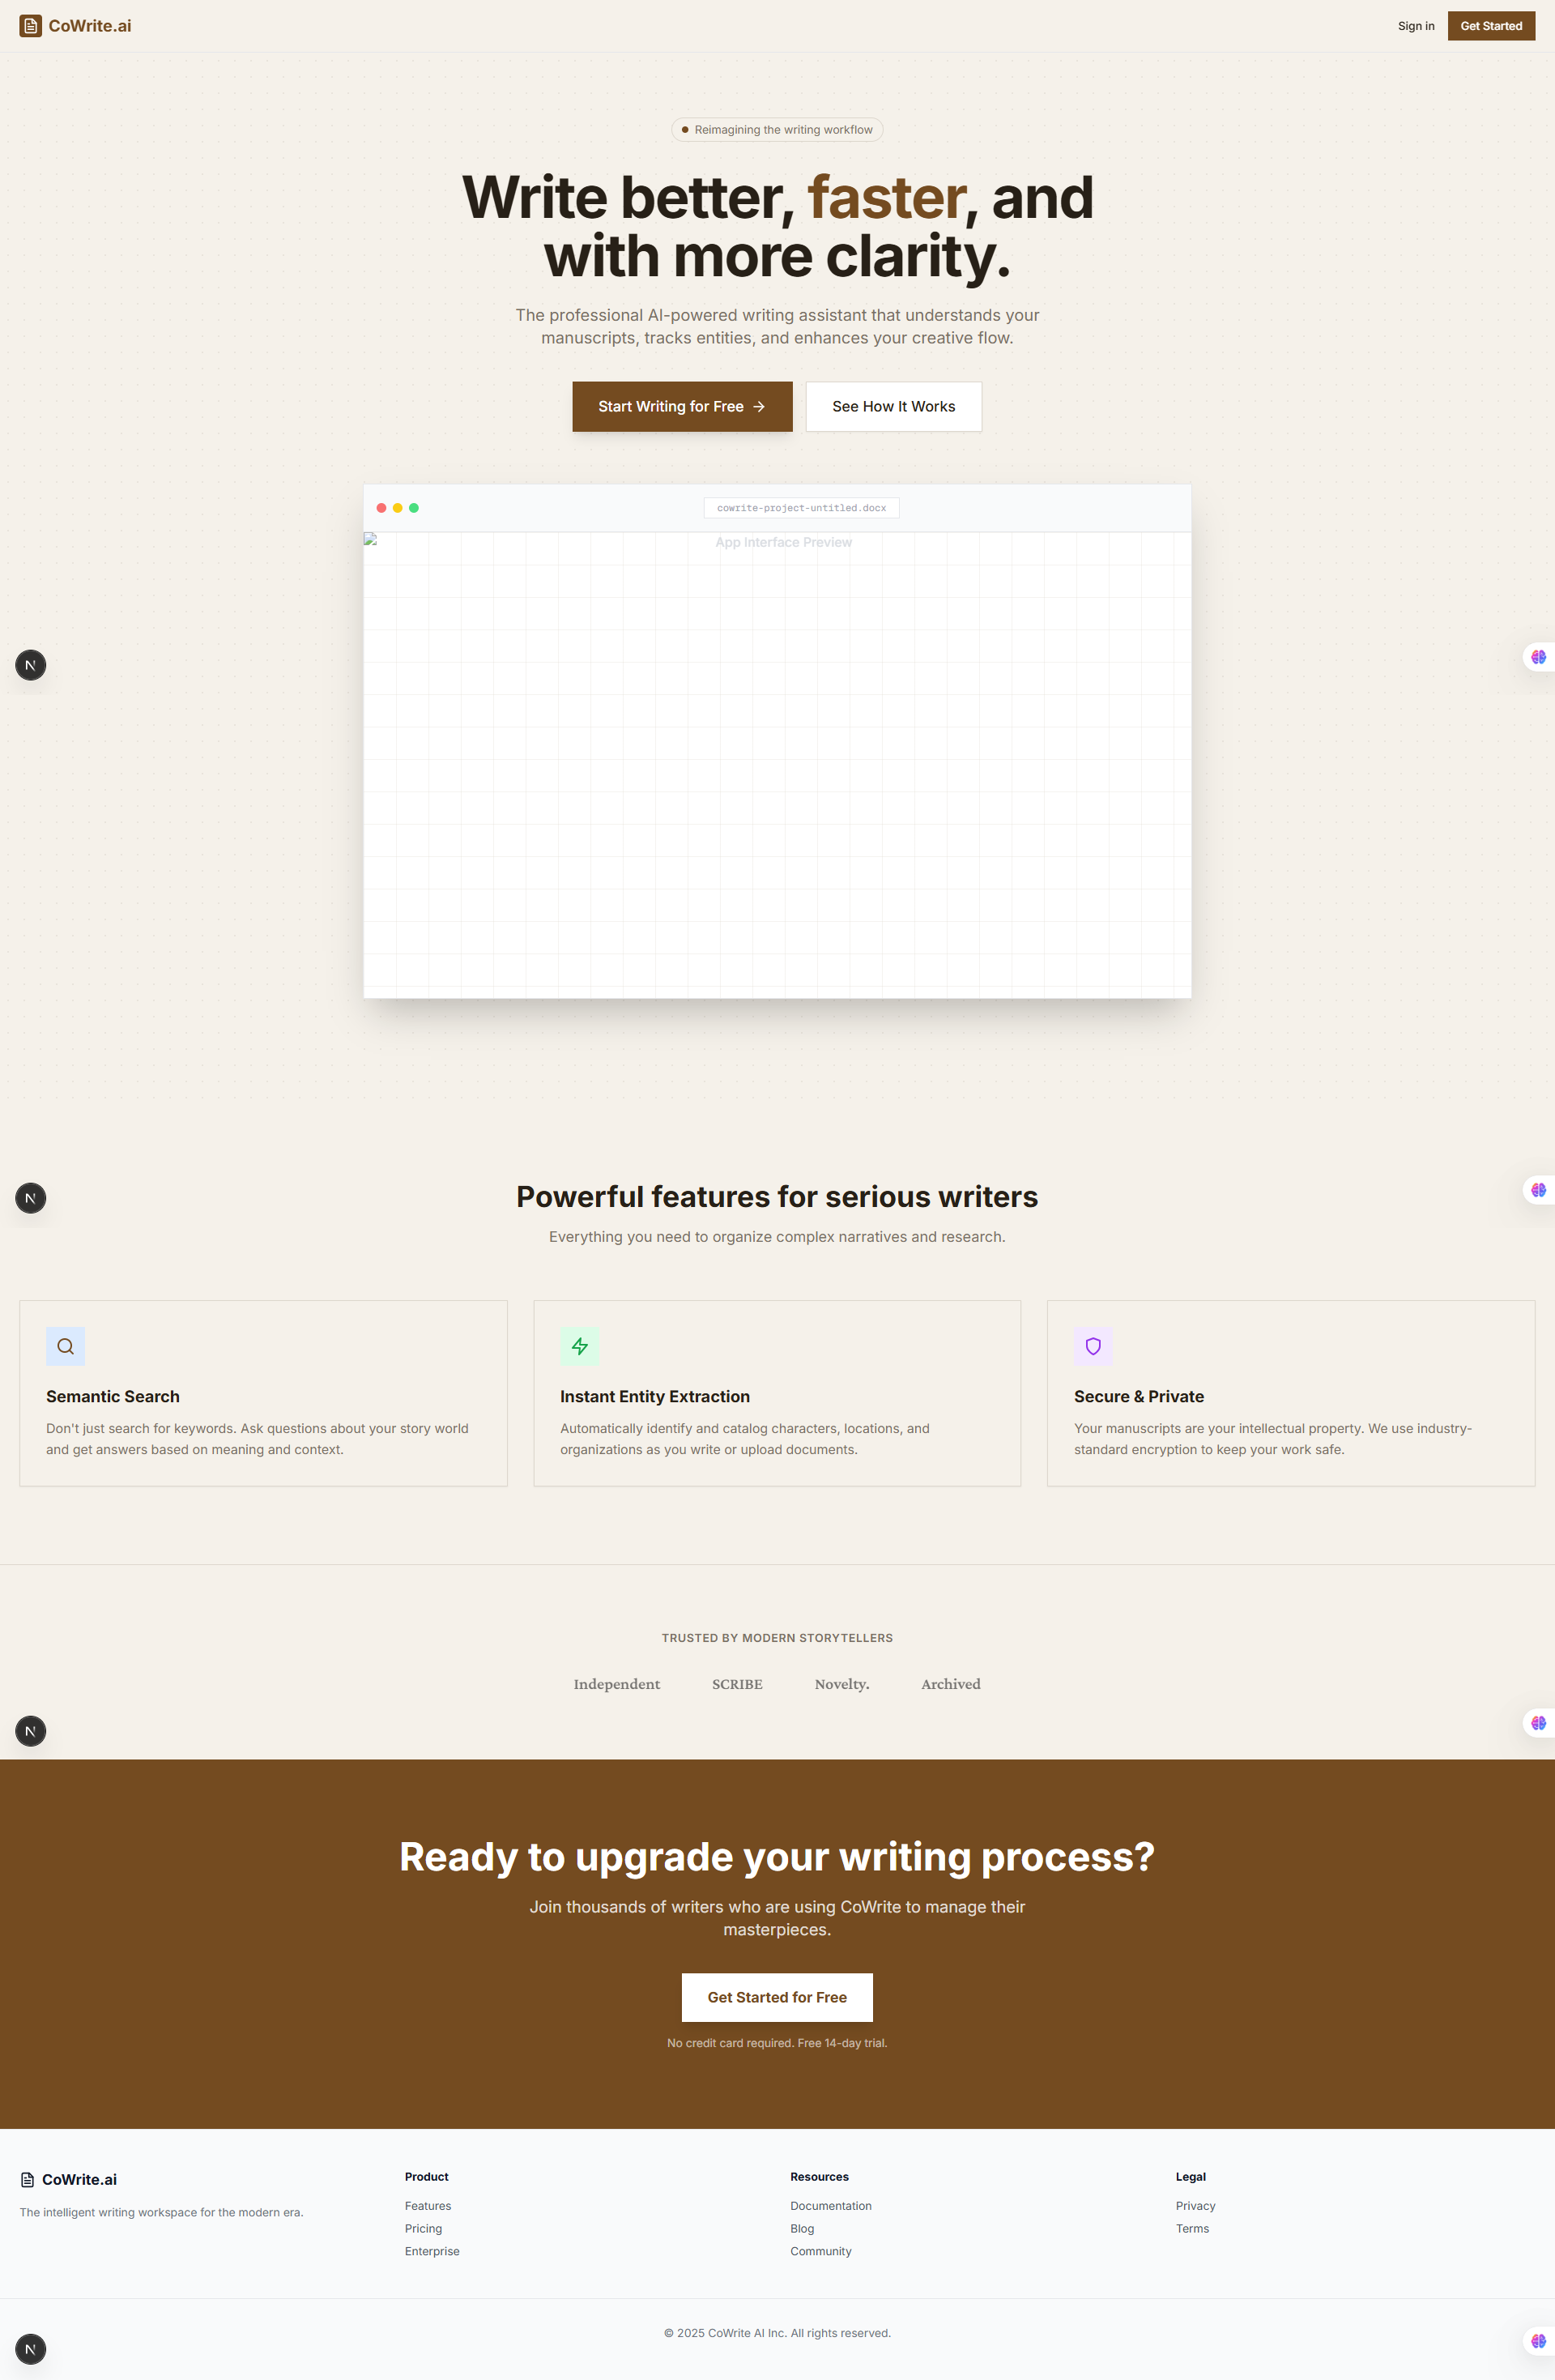
\includegraphics[width=\textwidth]{images/ui_1.png}
    \caption{CoWriteIA Landing Page}
    \label{fig:ui1}
\end{figure}

\subsection{Dashboard Interface}
\begin{figure}[H]
    \centering
    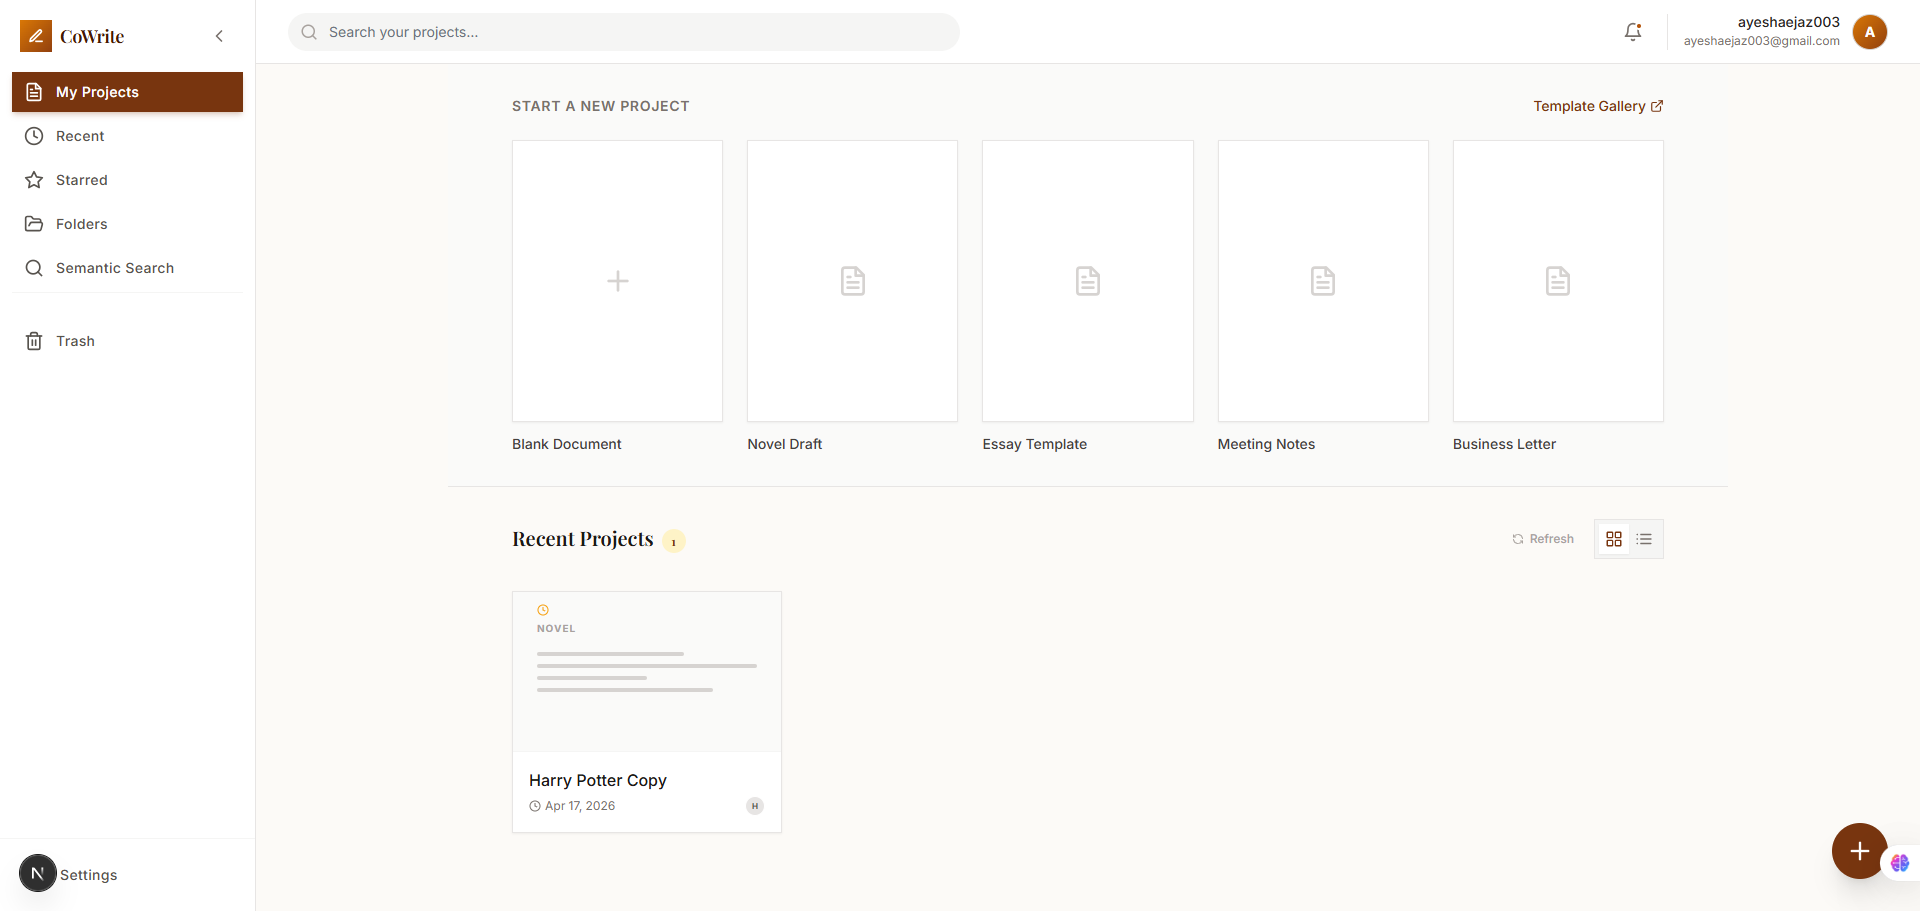
\includegraphics[width=\textwidth]{images/ui_2.png}
    \caption{CoWriteIA Dashboard Interface}
    \label{fig:ui1}
\end{figure}

\subsection{Writing Environment Interface}
\begin{figure}[H]
    \centering
    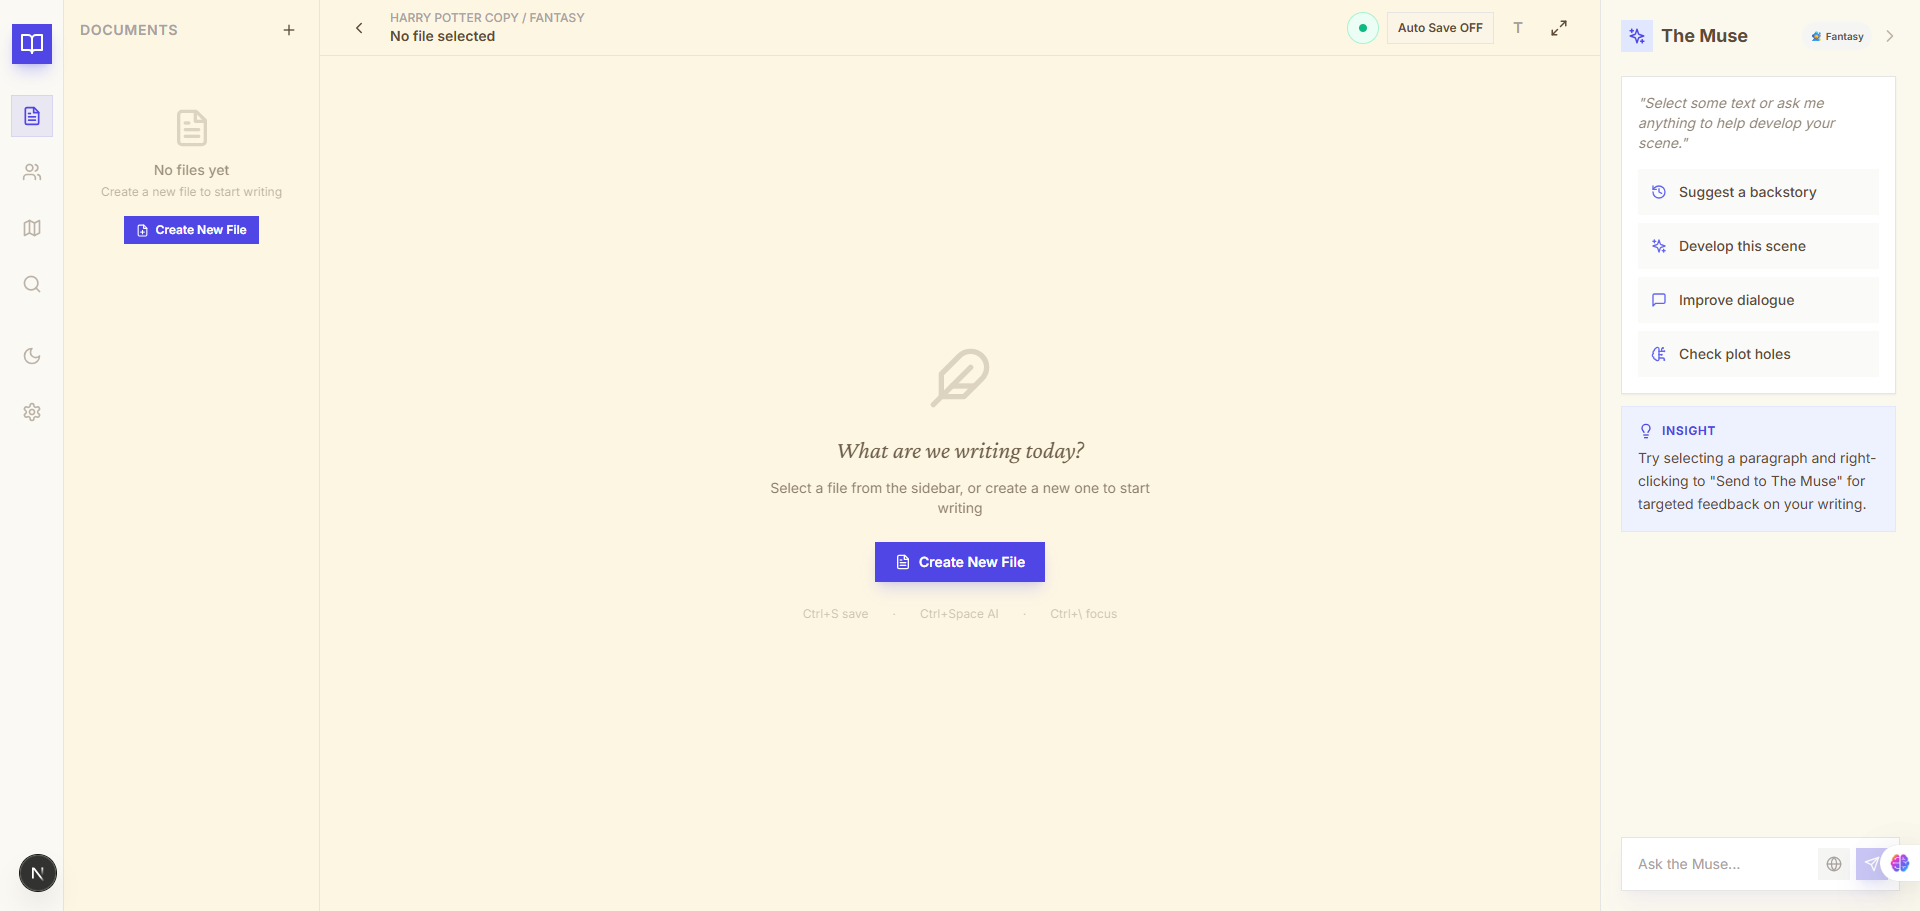
\includegraphics[width=\textwidth]{images/ui_3.png}
    \caption{Writing Environment Interface}
    \label{fig:ui2}
\end{figure}

\subsection{Writing Assistant Interface}
\begin{figure}[H]
    \centering
    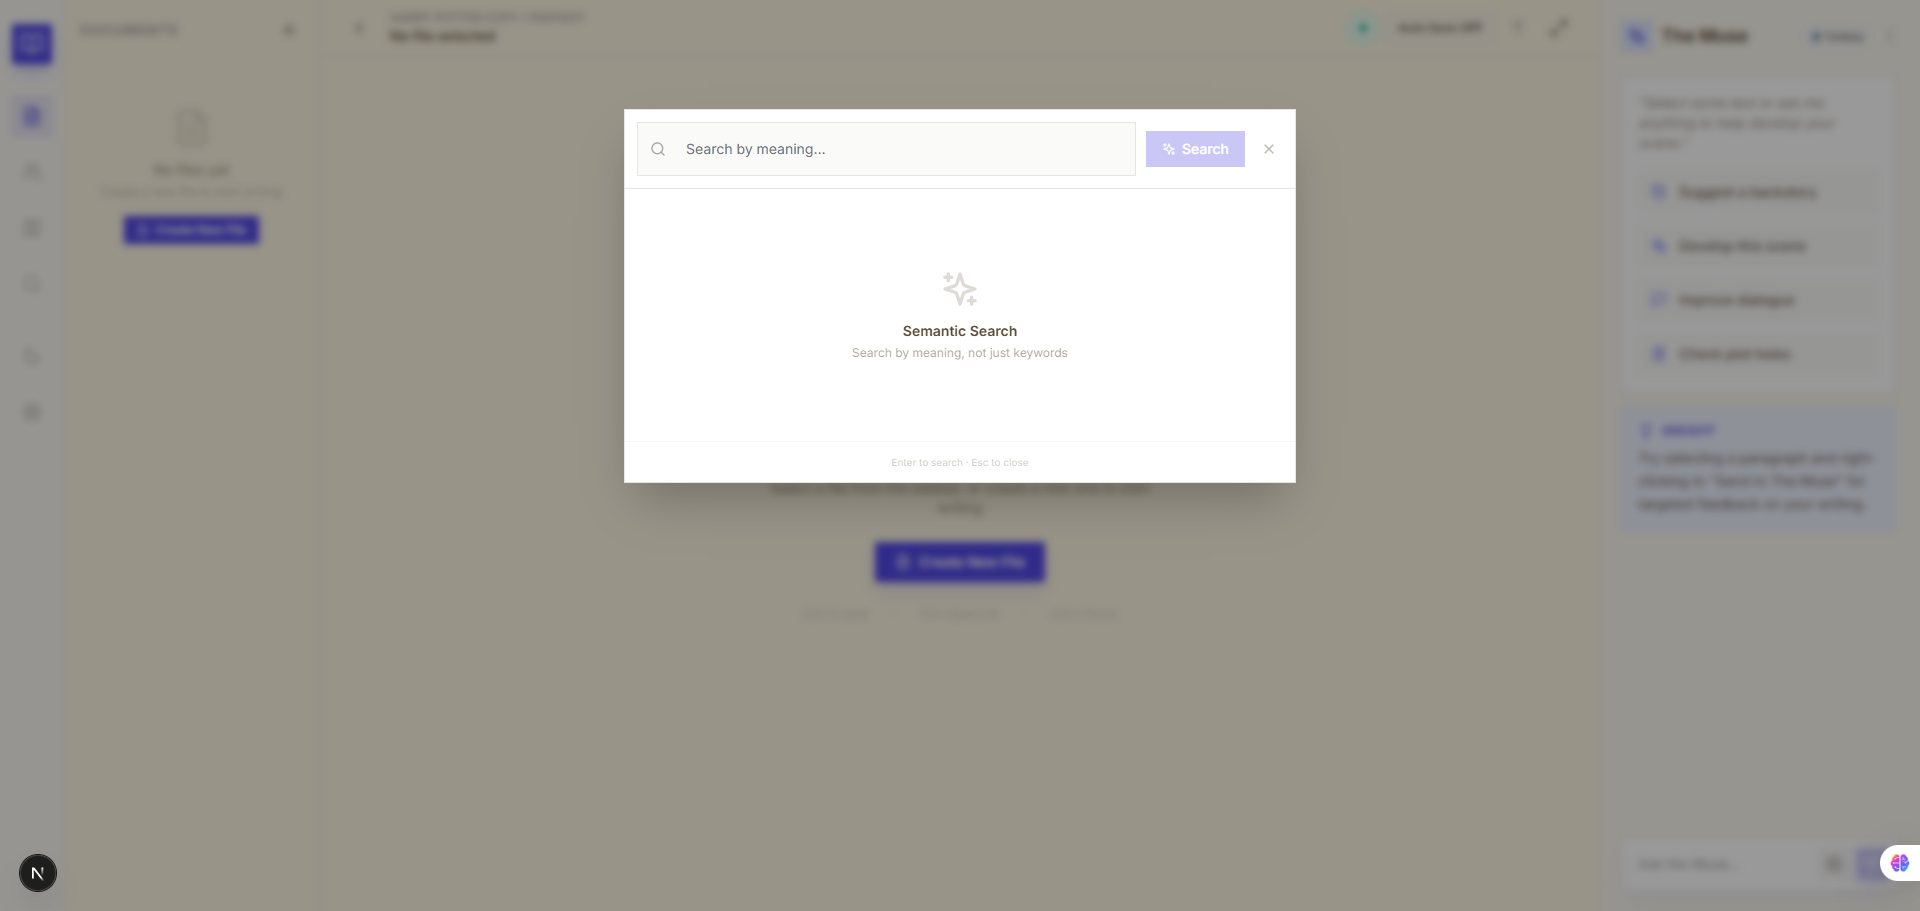
\includegraphics[width=\textwidth]{images/ui_4.png}
    \caption{Writing Assistant Interface}
    \label{fig:ui3}
\end{figure}

\subsection{Login Interface}
\begin{figure}[H]
    \centering
    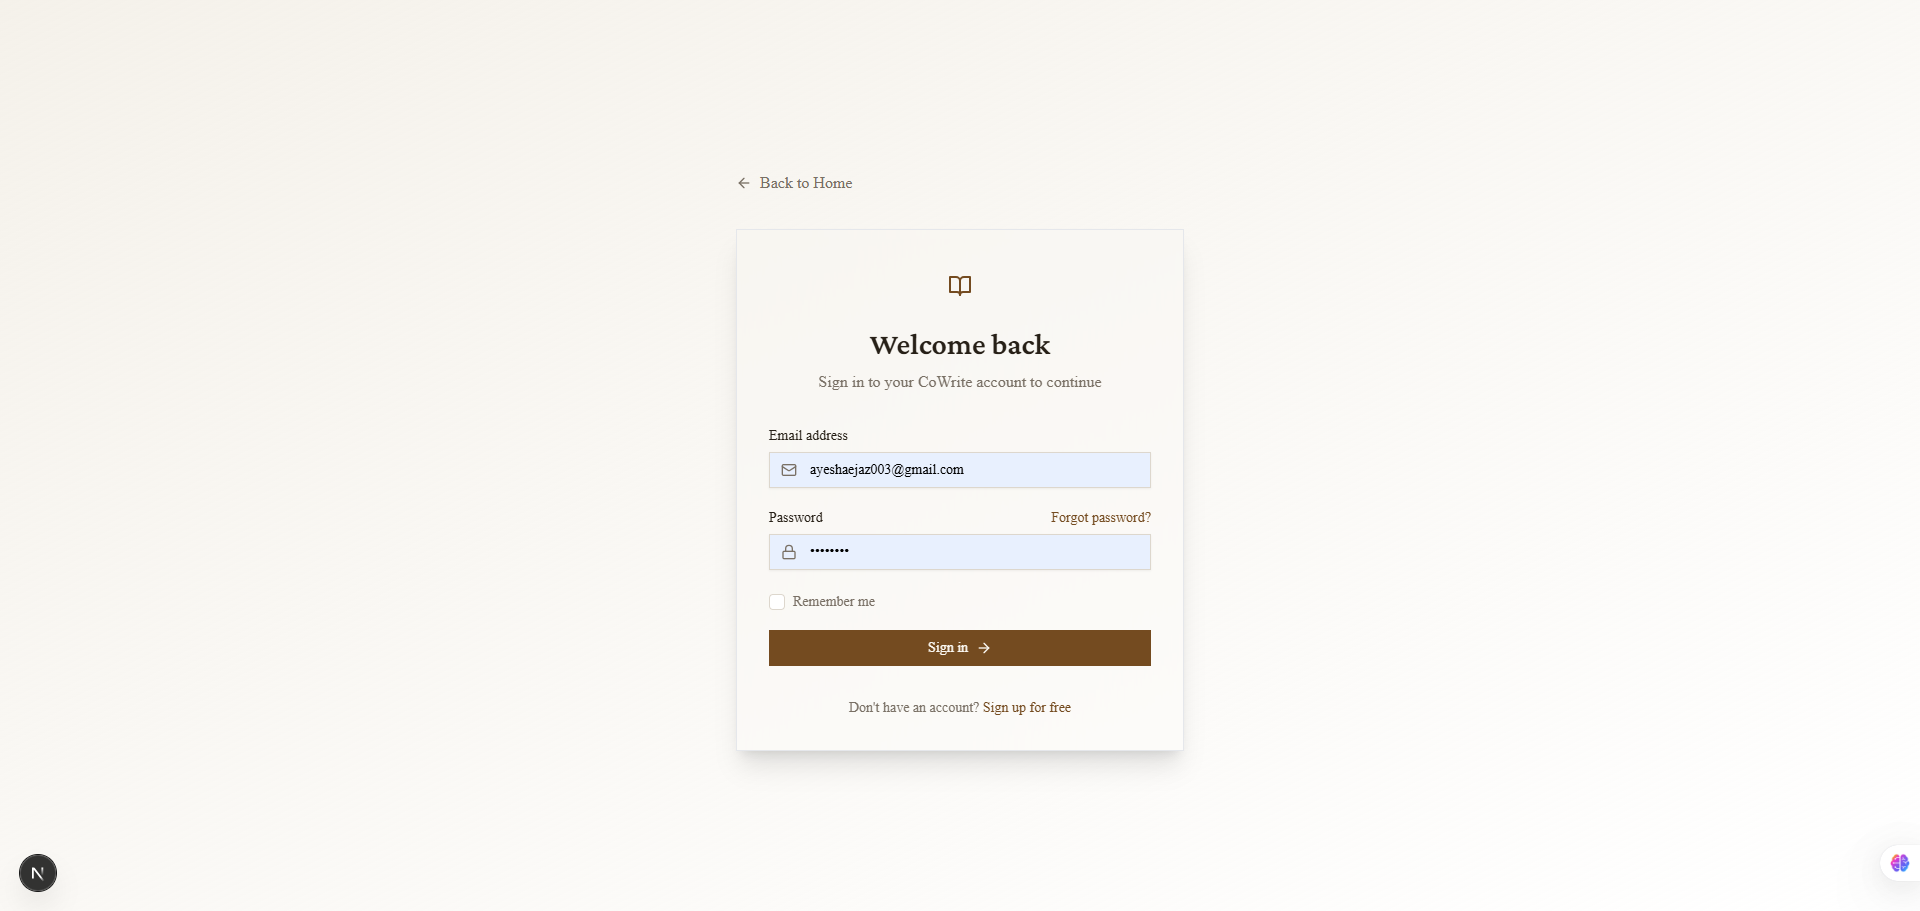
\includegraphics[width=\textwidth]{images/ui_5.png}
    \caption{Login Interface}
    \label{fig:ui4}
\end{figure}

\section{Appendix D: Detailed Use Case Specification}

\subsection{UC-01: Generate Context-Aware Writing}

\begin{table}[H]
\centering
\begin{tabular}{|p{3cm}|p{13cm}|}
\hline
\textbf{Use Case ID} & UC-01 \\ \hline
\textbf{Use Case Name} & Generate Context-Aware Writing \\ \hline
\textbf{Primary Actor} & Writer (User) \\ \hline
\textbf{Secondary Actors} & AI Processing Engine, Semantic Retrieval Module \\ \hline
\textbf{Preconditions} & 
\begin{itemize}
    \item User is authenticated and logged into the system.
    \item A project exists with at least one uploaded or created document.
    \item Project content has been indexed and embeddings are stored.
\end{itemize} \\ \hline

\textbf{Postconditions} &
\begin{itemize}
    \item AI-generated content is displayed to the user.
    \item Generated text may be saved to the project document.
\end{itemize} \\ \hline

\textbf{Trigger} & 
User selects the ``Generate Content'' option within the writing interface. \\ \hline

\textbf{Main Flow} &
\begin{enumerate}
    \item User opens a project document in the writing environment.
    \item User requests content generation (e.g., continue writing, rewrite, expand).
    \item System retrieves relevant context using semantic search.
    \item System sends the prompt + context to the AI model.
    \item AI model generates new content.
    \item System displays the generated text to the user.
    \item User may choose to accept, edit, or regenerate the content.
\end{enumerate} \\ \hline

\textbf{Alternate Flow} &
\begin{enumerate}
    \item[AF-1] User requests generation with no specific prompt.
    \begin{enumerate}
        \item System uses recent document content as context.
        \item AI generates a default continuation.
    \end{enumerate}
    \item[AF-2] User modifies the context manually.
    \begin{enumerate}
        \item User provides custom text or notes.
        \item System merges custom context with retrieved chunks.
    \end{enumerate}
\end{enumerate} \\ \hline

\textbf{Exceptions} &
\begin{enumerate}
    \item[E1] No embeddings found: System prompts user to index project files.
    \item[E2] AI service unavailable: System displays fallback message and suggests retrying.
    \item[E3] Empty or invalid user request: User is asked to refine or re-enter the prompt.
\end{enumerate} \\ \hline

\textbf{Priority} & High \\ \hline
\textbf{Frequency of Use} & Very frequent (core functionality) \\ \hline
\end{tabular}
\caption{Detailed Use Case: Generate Context-Aware Writing}
\label{tab:usecase-uc01}
\end{table}

\section{Appendix E: Pseudo-API Snippets (Call Signatures)}
\label{sec:appendix-e-pseudo-api}

{\small
\begin{itemize}
    \item \texttt{TextExtractionService.chunk\_text(file\_id: str,} \texttt{project\_id: str, text: str, start\_position: int = 0,} \texttt{start\_chunk\_index: int = 0) -> List[TextChunk]}
    \item \texttt{EmbeddingService.generate\_single\_embedding(text: str)} \texttt{-> List[float]}
    \item \texttt{EmbeddingService.generate\_embeddings(texts: List[str])} \texttt{-> List[List[float]]}
    \item \texttt{EmbeddingService.store\_text\_chunks\_with\_embeddings(} \texttt{file\_id: str, project\_id: str, chunk\_data: List[Dict])} \texttt{-> List[TextChunk]}
    \item \texttt{ChromaService.add\_embeddings(project\_id: str,} \texttt{entries: List[Dict]) -> None}
    \item \texttt{ChromaService.search\_similar(project\_id: str,} \texttt{query\_embedding: List[float], n\_results: int)} \texttt{-> List[Dict]}
    \item \texttt{RAGContextService.assemble\_context(query: str,} \texttt{project\_id: str, file\_id: Optional[str] = None,} \texttt{max\_chunks: int = 5) -> Dict}
    \item \texttt{AIChatService.chat(request: ChatRequest,} \texttt{user\_id: str) -> ChatResponse}
\end{itemize}
}